\chapter{Materiais e m�todos}

\begin{comment}
\documentclass[a4paper,11pt]{article}
\usepackage{graphicx}
\usepackage[brazilian]{babel}
\usepackage[latin1]{inputenc}
\usepackage[T1]{fontenc}
\usepackage{fullpage}
\usepackage{amsmath, amsthm, amssymb, bm}
\usepackage[ruled,vlined,portugues]{algorithm2e}
\usepackage{array}


\numberwithin{equation}{section}
\numberwithin{figure}{section}

\begin{document}
\end{comment}

\newcommand{\hx}{$h(\bar{\bf{x}})$}

\chapter{Modelos de Observa��o dos Sonares}\label{subsec:modelosonares}
\todo[inline]{Revisar a nota��o matem�tica das equa��es do sonar}
No contexto de localiza��o rob�tica, um modelo de observa��o � usado para representar o comportamento de sensores e, em especial, como as medidas obtidas se relacionam com grandezas do ambiente observado. 

Como descrito na se��o \ref{subsec:arqloc}, a localiza��o bayesiana por filtro de Kalman estendido utiliza as informa��es dos sensores para corrigir a do estado atual. Essencialmente, a informa��o utilizada pelo filtro � a diferen�a entre a observa��o esperada (aqui indicada por $h(\hat{\bf{x}})$, onde $\hat{\bf{x}}$ � a estimativa da postura) e a observa��o real (denotada por $z$). Por exemplo, suponha um rob� equipado com um sonar que incide perpendicularmente � uma parede, como na figura \ref{fig:exemplo_modelo}. Se ele estima estar em uma posi��o tal que a leitura esperada do sonar � 100 cm, mas a observa��o real � 80 cm, sabe-se que o rob� est� de fato mais perto da parede do que acredita. O papel do modelo de observa��o de um sensor � gerar as estimativas de observa��o \hx.

\begin{figure}[b]
	\centering
		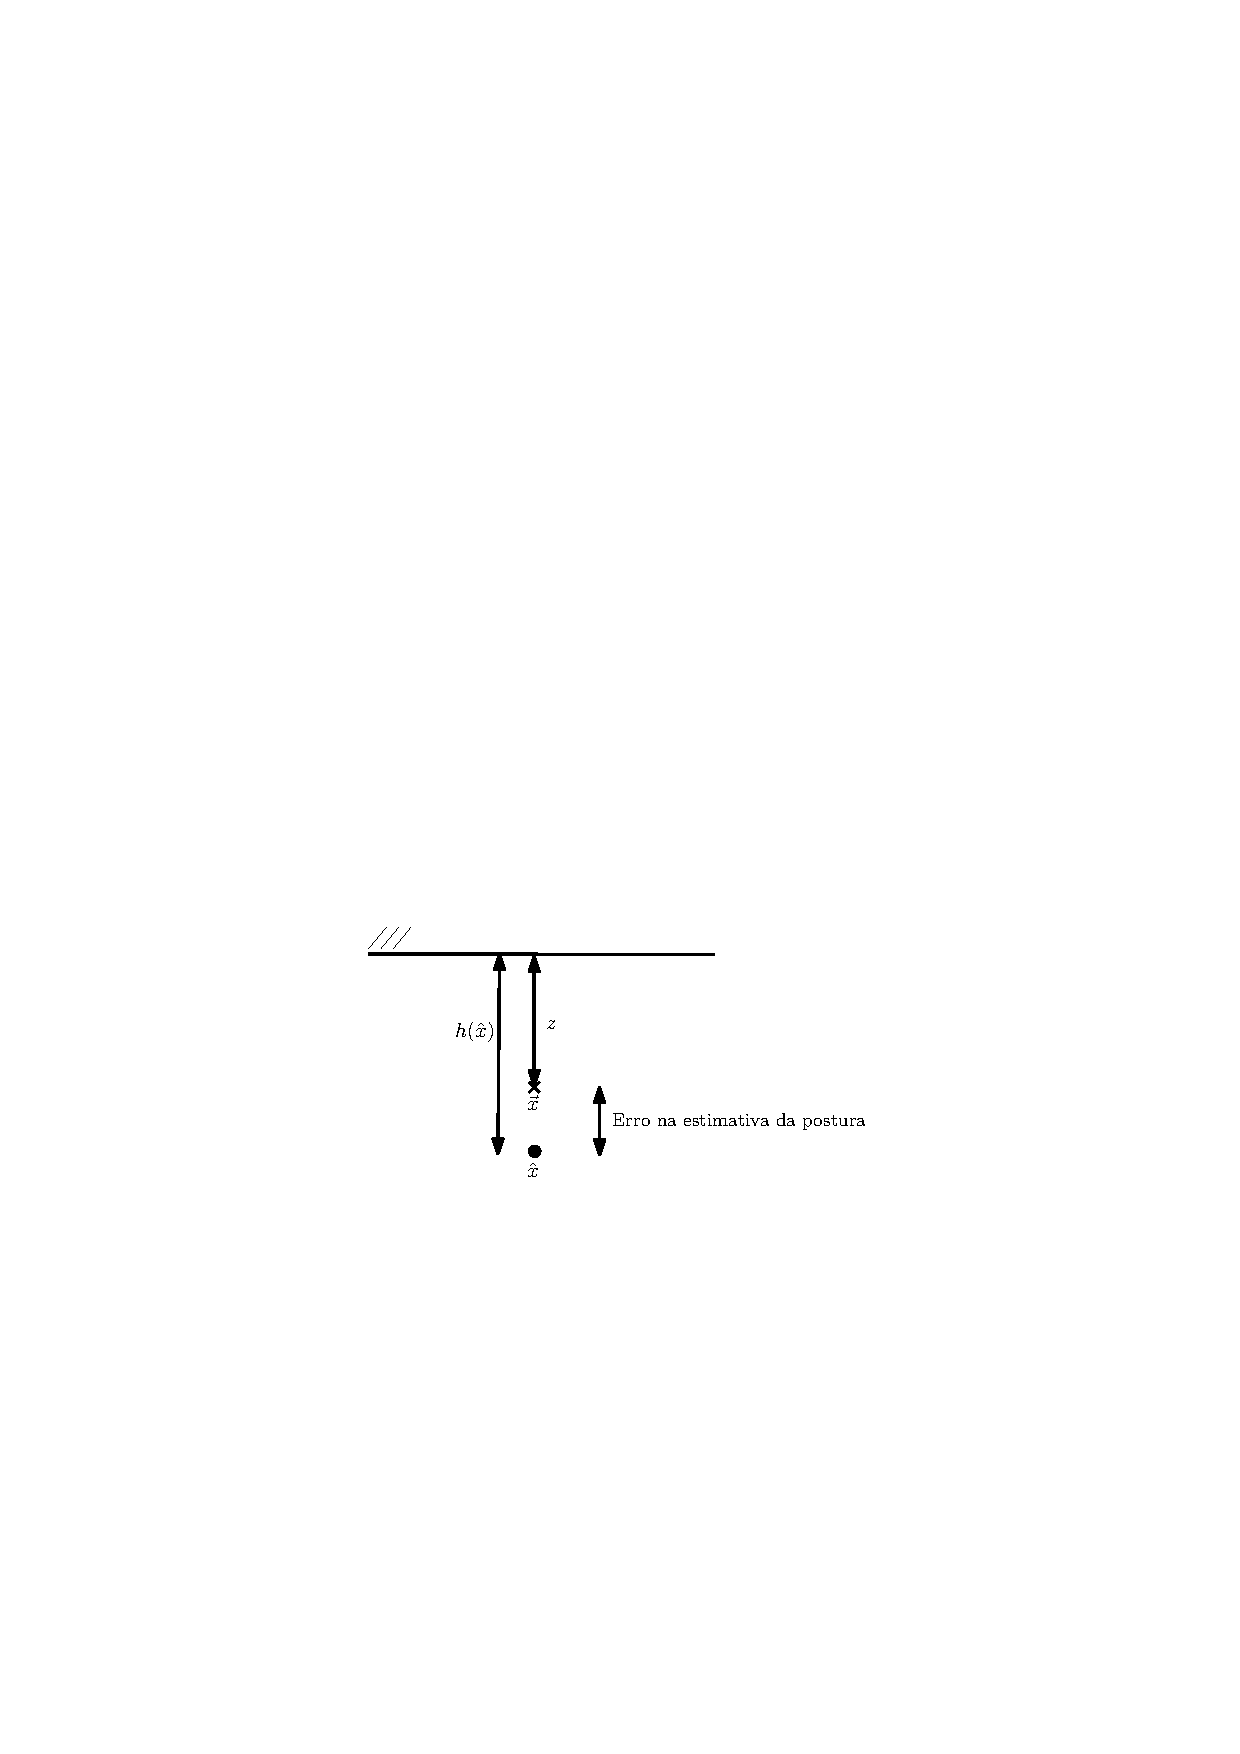
\includegraphics{imagens/sonar/exemplo_modelo.pdf}
			\caption{Um modelo de observa��o � usado para estimar o erro entre a postura real ($\vec{x}$) e a postura estimada ($\hat{\bf{x}}$). Neste exemplo, um sonar perpendicular � parede recebe leitura $z$, mas o modelo de observa��o prev�, para a posi��o estimada $\hat{\bf{x}}$, a leitura \hx. Essa diferen�a ser� utilizada pelo EKF para corrigir a predi��o da postura.}
	\label{fig:exemplo_modelo}
\end{figure}

Foram desenvolvidos dois modelos de observa��o dos sonares. O sonar � um sensor de profundidade que emite ondas sonoras e, a partir do tempo entre emiss�o e recep��o, calcula a dist�ncia ao obst�culo mais pr�ximo. Ele opera de maneira similar a um sensor laser, mas com menor precis�o e densidade. Contudo, um sensor laser � muito caro para algumas aplica��es. Um dos objetivos deste projeto � construir um rob� de baixo custo, utilizando sensores simples, de modo que a escolha do sonar se faz adequada.

\section{Modelo Baseado em Associa��es}
\label{sec:nossosonar}
A se��o \ref{subsec:sonarbarra} apresentou o modelo de observa��o desenvolvido em \cite{barra}. O modelo de observa��o baseado em associa��es � uma modifica��o desse modelo. Em particular, as equa��es foram refeitas para incluir o efeito do �ngulo relativo de cada sonar em rela��o ao centro do rob�, e a manuten��o de associa��es j� realizadas foi facilitada atrav�s do m�todo de rastreamento de paredes.

Este modelo � chamado de baseado em associa��es porque, antes de gerar observa��es esperadas e corrigir a postura predita, � necess�ria a confirma��o de que um sonar est� de fato observando uma determinada parede. A tarefa de relacionar as �ltimas leituras com uma parede do mapa chama-se associa��o. A principal motiva��o de um modelo deste tipo � diminuir os erros causados pelos sonares, dispositivos imprecisos.

De modo geral, a opera��o deste modelo pode ser dividida em quatro etapas. Primeiramente, as �ltimas $k$ observa��es s�o validadas e � determinado se uma parede est� sendo vista pelo sonar. Se isso for verdade, consulta-se o mapa do ambiente de modo a se associar as leituras mais recentes a uma parede no mapa. Por fim, quando a associa��o � realizada com sucesso, determina-se a observa��o que seria esperada para a postura estimada do rob�. A associa��o � registrada e o modelo tenta mant�-la nas pr�ximas itera��es, atribuindo uma pontua��o para seu grau de confian�a.

\paragraph{Valida��o das observa��es} As �ltimas $k$ observa��es s�o armazenadas, juntamente com a postura estimada em cada uma delas. Determina-se, atrav�s de um teste estat�stico, se as observa��es podem corresponder a uma superf�cie plana. Tamb�m nesta fase, curvas realizadas pelo rob� s�o detectadas. Nesse caso, o \textit{buffer} � limpo e a associa��o atual, se houver, � desfeita.

\paragraph{Associa��o das Observa��es com o Mapa} O mapa � ent�o consultado para encontrar uma parede que corresponda �s observa��es validadas. O processo � bastante conservador. Se o algoritmo de correspond�ncia encontrar uma, e somente uma, parede que corresponda �s leituras do sonar, a associa��o � realizada com sucesso.

\paragraph{Rastreamento de Associa��es} Caso uma associa��o seja realizada com sucesso, d�-se in�cio ao processo de rastreamento dessa associa��o. Para as pr�ximas leituras realizadas pelo sonar, a etapa de associa��o das observa��es n�o � executada - ou seja, o mapa n�o � consultado e assume-se que a parede observada � aquela que est� sendo rastreada. Estabelece-se uma pontua��o para cada rastreamento, em fun��o do erro entre as observa��es esperadas e obtidas. Quando a pontua��o se torna negativa, o rastreamento se encerra.

\paragraph{Obten��o das Observa��es Esperadas} De posse da parede que o sonar est� enxergando e da postura estimada do rob�, retorna-se a leitura esperada do sonar.

Cada uma destas etapas ser�o detalhadas nas pr�ximas se��es.

\subsection{Valida��o das Observa��es}
\label{sec:validacao}
Define-se $k$ como o n�mero de observa��es coletadas pelo sonar, e $k_{min}$ como o n�mero m�nimo de observa��es para que seja poss�vel a valida��o de uma superf�cie plana. Enquanto $k<k_{min}$ a valida��o falhar�. Quando $k=k_{min}$, inicia-se o processo de valida��o.

Para determinar se as �ltimas $k$ observa��es correspondem a uma parede, calcula-se a rela��o entre a diferen�a entre observa��es sucessivas e a dist�ncia percorrida pelo rob� entre elas, em movimento ret�lineo. A figura \ref{fig:modelo_sonar} ilustra que, caso um sonar esteja observando uma superf�cie plana, as leituras do sensor se alinhar�o em um segmento de reta. Isso equivale a dizer que a rela��o entre as diferen�as de leituras consecutivas e a dist�ncia percorrida entre essas leituras � constante. Matematicamente, seja $z_{i,j} = z^{(i)} - z^{(j)}$ a diferen�a entre duas medidas sucessivas e $d_{i,j}$ a dist�ncia percorrida entre elas, ent�o:

\begin{equation}
\frac{z_{2,1}}{d_{2,1}} = \frac{z_{3,2}}{d_{3,2}} = \dots = \frac{z_{i,j}}{d_{i,j}} = \gamma
\end{equation}

Idealmente, a rela��o � perfeita e $\frac{z_{i,j}}{d_{i,j}} = \gamma$ para quaisquer $i$ e $j$. Naturalmente, erros de medida introduzem varia��es nas observa��es, de modo que:

\begin{equation}
\frac{z_{2,1}}{d_{2,1}} = \gamma_{2,1} \approx \frac{z_{3,2}}{d_{3,2}} = \gamma_{3,2} \approx \dots \approx \gamma_{i, j}
\end{equation}

\begin{figure}
	\centering
		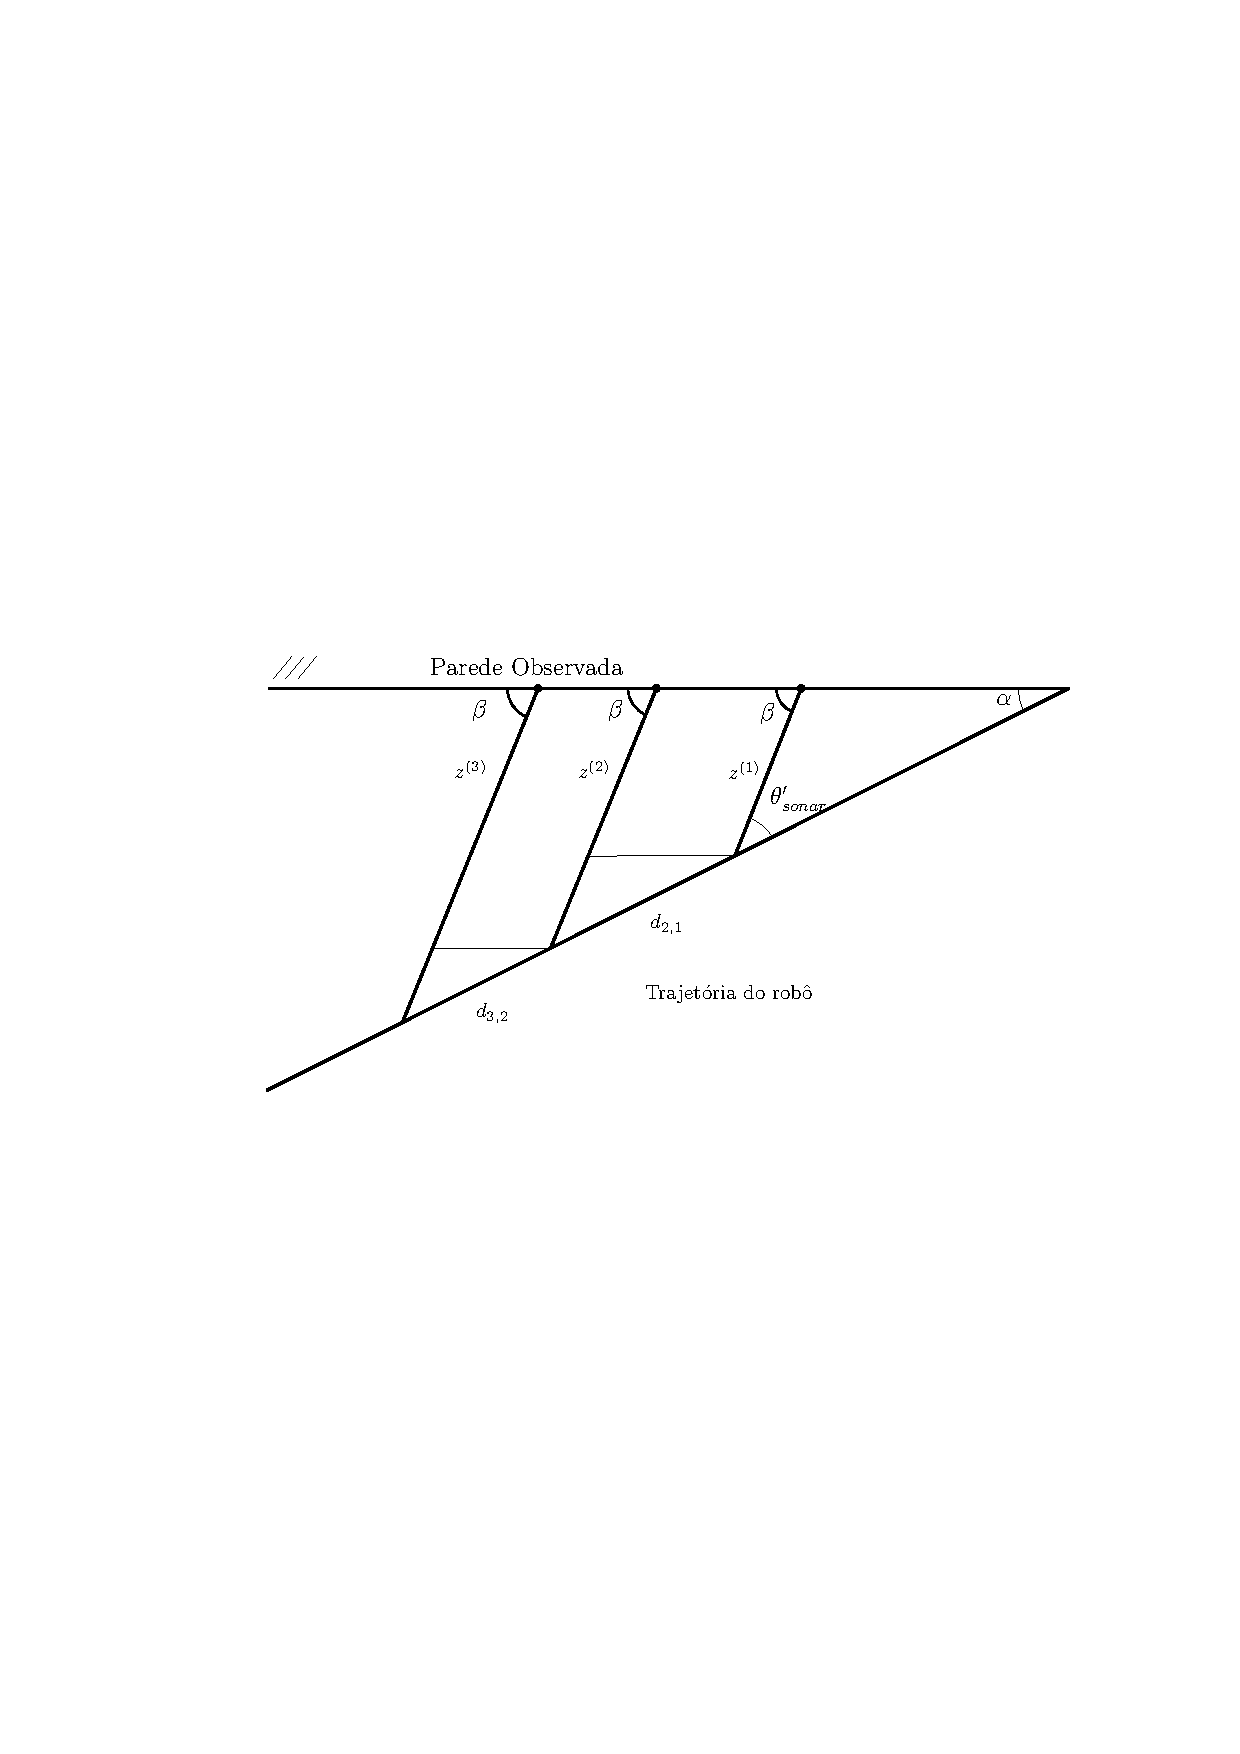
\includegraphics{imagens/sonar/modelo_sonar.pdf}
		\caption{Representa��o das observa��es de um sonar com �ngulo relativo $\theta'_{sonar}$. Os feixes do sonar incidem na parede com um �ngulo $\beta$. Cada $z^{(i)}$ � uma observa��o, e $d_{i,j}$ � a dist�ncia percorrida entre as observa��es $i$ e $j$. Como a parede � uma superf�cie plana, a rela��o entre a diferen�a das leituras e a dist�ncia percorrida � constante.}
	\label{fig:modelo_sonar}
\end{figure}

Assumindo-se que um �nico segmento de reta est� sendo visto (uma mesma parede) em todas as $k$ observa��es, podemos considerar que todos os elementos do conjunto formado por $\gamma$ s�o elementos de uma mesma distribui��o normal. Se isso for verdade, as observa��es s�o validadas e passa-se � pr�xima fase do modelo de observa��o. O seguinte teste de hip�tese pode ser utilizado para averiguar se o conjunto de $\gamma_{i,j}$ corresponde a uma distribui��o normal:

\begin{equation*}
		H_{0}:\gamma ~ N(A, \sigma^{2}_{obsmedia})
\end{equation*}
\begin{equation*}
		H_{1}:\gamma ~ N(A, \sigma^{2}_{alternativo}), \sigma^{2}_{obsmedia} < \sigma^{2}_{alternativo}
\end{equation*}
sendo que o teste � realizado sobre a estat�stica $\chi^{2}$.
Para aceitar $H_{0}$, � verificado se $\chi^{2}$ � menor que um dado limite:
\begin{equation}
	\chi^{2}_{k-2} < \chi^{2}_{k-2,\alpha}
	\label{eq:chitest}
\end{equation}
onde o segundo termo � tabelado, $\alpha$ indica a confian�a no teste e o primeiro termo � obtido da seguinte equa��o:
\begin{equation*}
	\chi^{2}_{k-2} = \frac{(k-2)s^{2}_{\gamma}}{\sigma^{2}_{obsmedia}}
\end{equation*}
onde $s^{2}_{\gamma}$ � a vari�ncia do conjunto formado pelos $\gamma_{i,i-1}$ de cada par de observa��es.

Considerando que todos os $\gamma_{i,i-1}$ pertencem � mesma distribui��o de probabilidades, $\sigma^{2}_{obsmedia}$ � a vari�ncia esperada dessa distribui��o. De acordo com \cite{barra}, seu valor � dado por:

\begin{equation}
\sigma^2_{obsmedia}=\sigma^2_{\gamma} = \vec{F}_\gamma \bm{\Sigma}_{\omega_{i,i-1}} \vec{F}_\gamma^{T} 
\end{equation}

\begin{align}
\vec{F}_\gamma=\frac{\partial\gamma(\omega_{i,i-1})}{\partial\omega_{i,i-1}}  |  \bm{\omega_{i,i-1}} = \bm{\bar{\omega}_{i,i-1}} = \notag \\
= \left( -\frac{(k-1)z_{i,i-1}}{d^{2}_{k,1}}~\frac{k-1}{d_{k,1}} \right) | \bm{\omega_{i,i-1}}
\end{align}

\begin{equation}
\bm{\Sigma}_{\omega_{i,i-1}} =
\begin{pmatrix}
\frac{\sigma^2_{d_{k,1}}}{(k-1)^2} & E_z\left[ z_{i, i-1} \frac{d_{k,1}}{k-1} \right] \\
 E_z\left[ z_{i, i-1} \frac{d_{k,1}}{k-1}\right] & \sigma^2_{z_{i,i-1}}
\end{pmatrix}
\end{equation}

\begin{equation}
\sigma^2_{z_{i,i-1}}=2\sigma^2_{obs} + \frac{\sigma^2_{d_{k,1}}}{(k-1)^2} \sin^2(\alpha)
\end{equation}

\begin{equation}
 E_z\left[ z_{i, i-1} \frac{d_{k,1}}{k-1} \right] = \frac{\sigma^2_{d_{k,1}} \sin(\alpha)}{(k-1)^2}
\end{equation}

\begin{equation}
\bm{w_{i,i-1}}=
\begin{pmatrix}
\frac{d_{k,1}}{k-1} & z_{i,i-1}
\end{pmatrix}^T
\end{equation}
Nas equa��es acima, $d_{k,1}$ � a dist�ncia percorrida pelo rob� durante as �ltimas $k$ observa��es; $z_{i,j}$ � a diferen�a entre a leitura dos sonares nos instantes $i$ e $j$; $\sigma^2_{obs}$ � a incerteza da observa��o do sonar; $\sigma^2_{d_{k,1}}$ � a incerteza no deslocamento do rob� e vale $\frac{d_{k,1}\sigma_{desloc}}{k-1}$, com $\sigma_{desloc}$ determinado experimentalmente; e $\alpha$ � o �ngulo de incid�ncia do rob� com a parede observada. $\alpha$ pode ser calculado empiricamente do seguinte modo:

\begin{equation}
\sin \alpha=\frac{z_{k,1}\sin \theta'_{sonar}}{\sqrt{z_{k,1}^2 + d_{k,1}^2 - 2z_{k,1} d_{k,1} \cos \theta'_{sonar}}}
\label{eq:novoalpha}
\end{equation}

\subsection{Associa��o das observa��es com o mapa}\label{sec:associacao}
Se as $k$ observa��es armazenadas passarem no teste estat�stico da equa��o \ref{eq:chitest}, procede-se com a busca de uma parede mapeada que corresponda �s leituras validadas. O algoritmo utilizado trata as paredes como retas infinitas, definidas em termos de $r_{wall}$, o comprimento do segmento perpendicular � reta e que passa pela origem, e $\theta_{wall}$, o �ngulo deste segmento com rela��o � origem. A figura \ref{fig:retas} ilustra essa conven��o.

Duas etapas de elimina��o s�o aplicadas sobre as paredes do mapa, de modo a reduzir o espa�o de busca. Primeiramente, paredes que estejam fora do alcance do sonar s�o eliminadas; em seguida, paredes que estejam al�m do cone de vis�o do sonar tamb�m s�o desconsideradas.

\paragraph{Elimina��o de paredes distantes}

Para cada parede do mapa, representada em termos de $r_{wall}$ e $\theta_{wall}$, calcula-se a dist�ncia perpendicular at� a �ltima posi��o predita do rob�, $\bar{\bf{{x}}}$. Caso essa dist�ncia seja maior do que um dado limite -- a faixa de opera��o do sonar utilizado --, rejeita-se esta parede como candidata a associa��o.

\paragraph{Elimina��o de paredes pelo �ngulo do sonar}

� necess�rio tamb�m eliminar as paredes candidatas pelo �ngulo de abertura do sonar. Neste caso, as paredes n�o s�o tratadas como retas infinitas, e sim como segmentos. Um segmento s� pode ser observado se um cone centrado na postura global do sonar com �ngulo de abertura $\phi$ interseccion�-lo. O algoritmo \ref{algo:cone} descreve o comportamento desta etapa.

\begin{figure}[hbt]
	\centering
	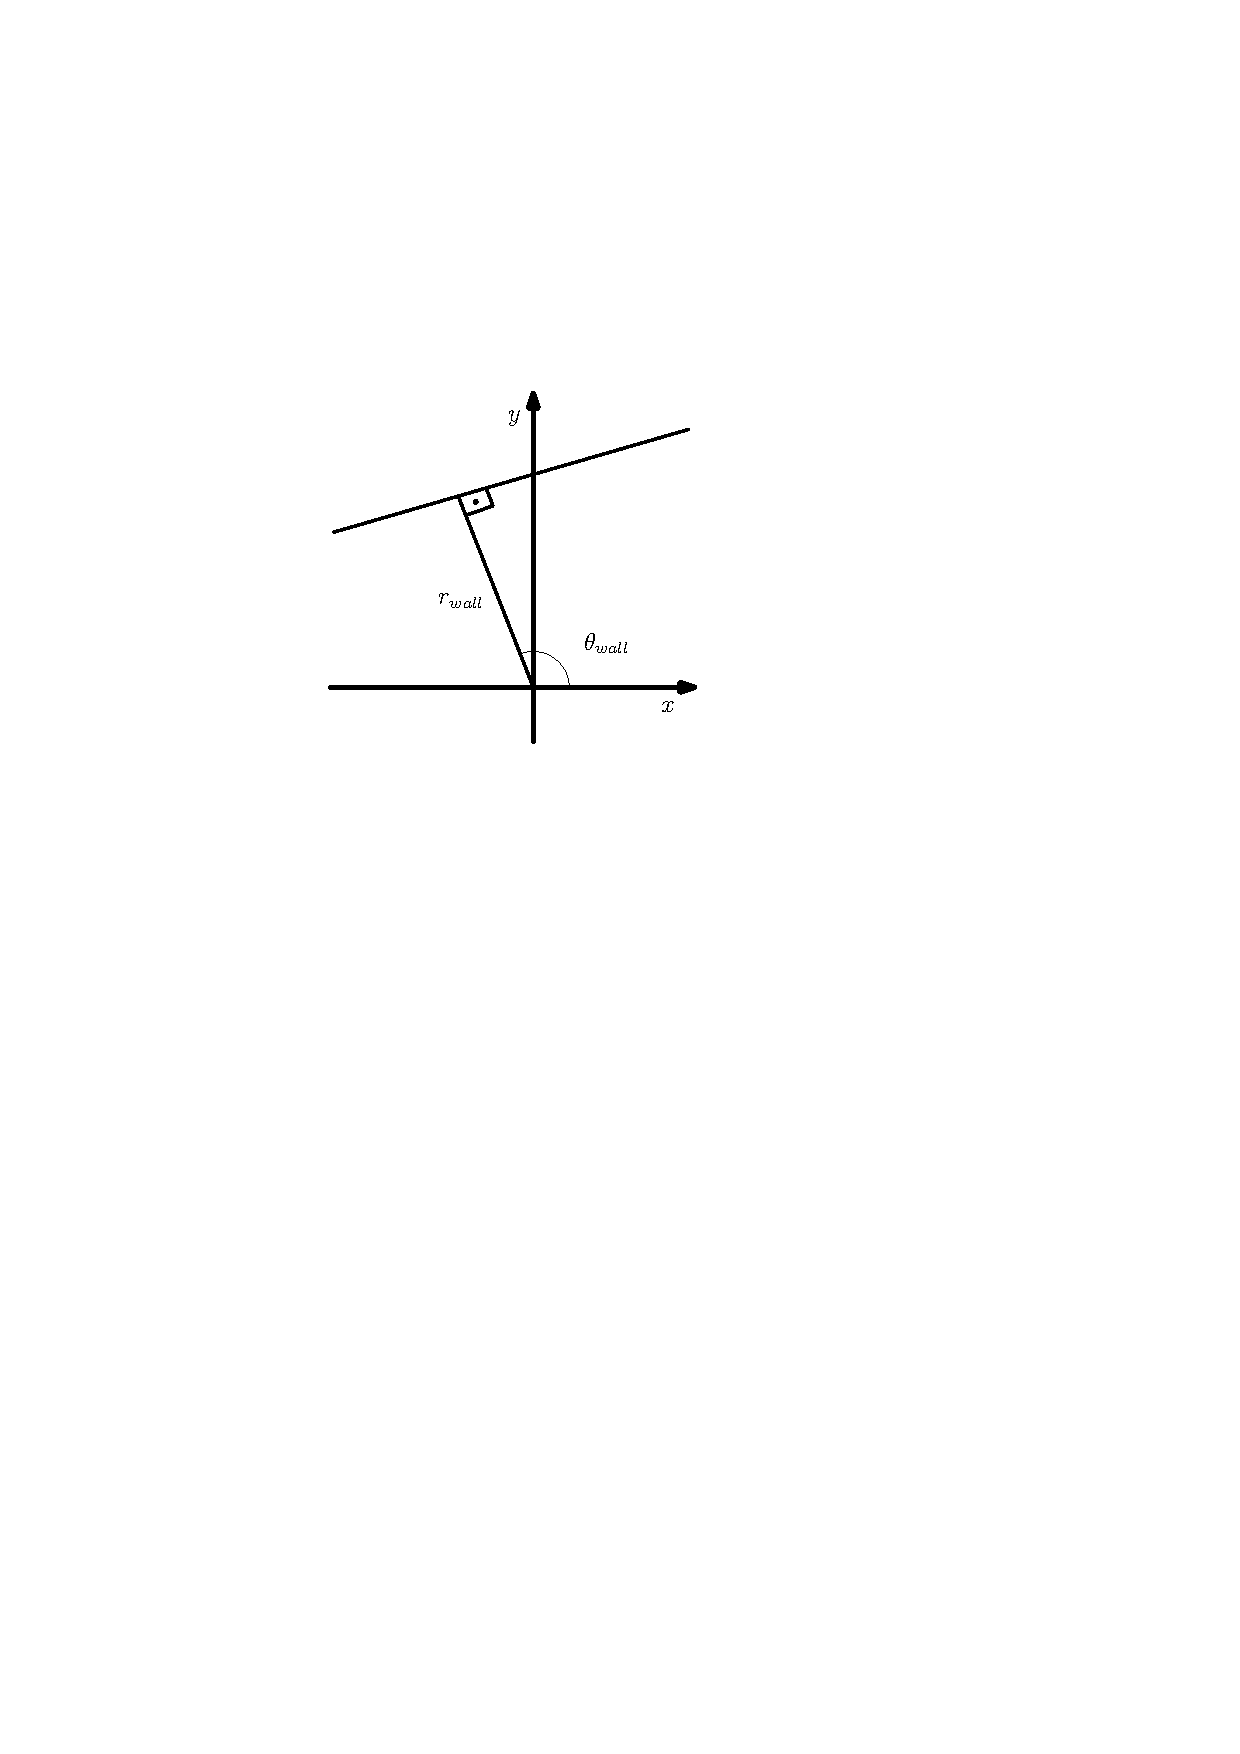
\includegraphics[width=.5\columnwidth]{imagens/retas.pdf}
	\caption{O modelo adotado para representar as paredes do mapa, que s�o tratadas como retas infinitas. Cada reta � definida em termos de $r_{wall}$ e $\theta_{wall}$.}
	\label{fig:retas}
\end{figure}

\begin{algorithm}
	\dontprintsemicolon
	\SetKwData{bordau}{borda1}
	\SetKwData{bordad}{borda2}
	\SetKwData{eixo}{eixo}
	\SetKwData{parede}{parede}
	\SetKwData{pareta}{retaParede}
	\SetKwData{verdade}{verdadeiro}
	\SetKw{e}{e}
	\SetKw{lp}{$($}
	\SetKw{rp}{$)$}
	\SetKw{ou}{ou}
	\SetKwData{falso}{falso}
	\SetKwData{interbu}{interse��oBorda1}
	\SetKwData{interbd}{interse��oBorda2}
	
	\Entrada{A postura global predita do sonar, $(\bar{x}_{sonar}, \bar{y}_{sonar}, \bar{\theta}_{sonar})$, e seu �ngulo de abertura, $\phi$}
	\Entrada{A parede, representada por um segmento de reta (\parede)}
	\Saida{\verdade se a parede for vis�vel pelo sonar; \falso caso contr�rio}
	
	\Inicio{
		\pareta $\leftarrow$ a reta que cont�m \parede \;
		\bordau $\leftarrow$ a semireta com origem em $(\bar{x}_{sonar}, \bar{y}_{sonar})$ e inclina��o $\bar{\theta}_{sonar} + \phi/2$ \;
		\bordad $\leftarrow$ a semireta com origem em $(\bar{x}_{sonar}, \bar{y}_{sonar})$ e inclina��o $\hat{\theta}_{sonar} - \phi/2$ \;
		\eixo $\leftarrow$ a semireta  com origem em $(\bar{x}_{sonar}, \bar{y}_{sonar})$ e inclina��o $\hat{\theta}_{sonar}$ \;
		\interbu $\leftarrow$ a interse��o, se existir, entre \bordau e \pareta \;
		\interbd $\leftarrow$ a interse��o, se existir, entre \bordad e \pareta \;
		\Se{\lp \interbu  \ou \interbd\ \rp \e \parede cont�m o ponto de interse��o}{\Retorna{\verdade} \;}
		\SenaoSe{\interbu \e \interbd}{
			\SetKwData{seginter}{segmentoInterse��es}
			\seginter $\leftarrow$ o segmento de reta que une as duas interse��es \;
			\lSe{ \seginter cont�m \parede }{\Retorna{\verdade}} \;
			\lSenao{\Retorna{\falso}}
		}
		\SenaoSe{ \interbu \ou \interbd } {
			\SetKwData{angpu}{anguloExtremo1}
			\SetKwData{angpd}{anguloExtremo2}
			\angpu $\leftarrow$ $atan2($\parede.extremo1.y, \parede.extremo1.x$)$ \;
			\angpd $\leftarrow$ $atan2($\parede.extremo2.y, \parede.extremo2.x$)$ \;
			\lSe{
			$distanciaAngular($ \eixo, \angpu $) \leq \phi / 2$ \ou 
			$distanciaAngular($ \eixo, \angpd $) \leq \phi / 2$}{\Retorna{\verdade} \;
			} \;	
		}
		\Senao{ \Retorna{\falso}}	
	}
	\caption{Algoritmo de elimina��o de uma parede pelo �ngulo do sonar}
		\label{algo:cone}
\end{algorithm}

As paredes que passarem por ambos as etapas s�o candidatas � associa��o. Para que se possa selecionar a parede correta, � calculada a observa��o esperada para aquela parede, supondo correta a predi��o $\bar{\textbf{x}}$. D�-se a essa observa��o esperada o nome de \hx, e seu c�lculo � explicado na se��o \ref{sec:obsesperada}. Averigua-se, ent�o, a diferen�a entre \hx e $z$, a observa��o mais recente obtida do sonar. A ideia � rejeitar associa��es que produzam erros grandes demais.


O teste realizado �:

\begin{equation}
\frac{(z-h(\bar{\bf{x}}))^2}{\sigma_{obs}^2} < g^2,
\label{eq:testeassoc}
\end{equation}

onde $\sigma_{obs}^2$ � a vari�ncia das medidas e $g^2$ � um limite determinado experimentalmente. Se uma, e somente uma, parede do mapa passar pelo teste da equa��o \ref{eq:testeassoc}, considera-se a associa��o realizada com sucesso. Nesse caso, o modelo � capaz de produzir uma observa��o esperada, de acordo com a equa��o \ref{eq:hx}, e d�-se in�cio � fase de rastreamento da associa��o.

\subsection{Rastreamento de associa��o}
Para a opera��o bem-sucedida do sistema de localiza��o, � importante fornecer dados frequentemente, de modo a se corrigir a postura estimada com rapidez. � para aumentar essa taxa de corre��es que se desenvolveu o modo de rastreamento de associa��o, que entra em vigor assim que uma associa��o entre leituras e parede � realizada com sucesso.

Uma associa��o sendo rastreada tem associada a si uma pontua��o num�rica, iniciada com um valor pr�-definido. A cada nova leitura gerada pelo sonar em um instante $t$, a pontua��o $p$ � recalculada, do seguinte modo:

\begin{equation*}
	\epsilon_{t} = (z_t-h(\bar{\bf{x}}_t))^2
\end{equation*}
\begin{equation*}
	\Delta_{\epsilon} = \epsilon_{t-1} - \epsilon_{t}
\end{equation*}
\begin{equation}
	p_t = p_{t-1} + K\Delta_{\epsilon},
\end{equation}

onde:

\begin{equation}
K = \left\{ 
\begin{array}{l l}
  K_{piora} & \quad \text{se $\Delta_{\epsilon} > 0$}\\
  K_{melhora} & \quad \text{se $\Delta_{\epsilon} < 0$}\\
\end{array} \right.
\end{equation}

A fun��o da pontua��o � representar a confian�a que se tem naquela associa��o. Se os erros entre a observa��o esperada e a observa��o real diminu�rem ou se mantiverem constantes, � sinal de que a associa��o n�o est� tendo efeito negativo, e aumenta-se a pontua��o. Por outro lado, se os erros estiverem aumentando, � desejado que a associa��o seja interrompida, pois � poss�vel que n�o se esteja mais observando a mesma parede. De modo geral, deseja-se que $K_{piora} > K_{melhora}$ para evitar associa��es err�neas.

A pontua��o de uma associa��o afeta tamb�m a covari�ncia do erro do modelo de observa��o, R:

\begin{equation}
R = \begin{bmatrix}
	R_{base} + \frac{C}{p}
\end{bmatrix},
\label{eq:matrizr}
\end{equation}

onde $R_{base}$ e $C$ s�o constantes ajustadas experimentalmente.

Quando a pontua��o de um rastreamento cai abaixo de zero, a associa��o � desfeita. Na pr�xima itera��o do algoritmo do modelo de observa��o do sonar, a fase de associa��o descrita na se��o \ref{sec:associacao} � realizada e, caso tenha sucesso, d�-se in�cio a um novo rastreamento.

\subsection{Obten��o da Observa��o Esperada}
\label{sec:obsesperada}
Conhecida a parede que se est� observando, o pr�ximo passo � fornecer ao EKF as seguintes informa��es: a observa��o esperada para a postura estimada, \hx; a observa��o real obtida, $z$; a matriz de covari�ncia, R e o jacobiano de \hx, a matriz G.

\paragraph{C�lculo da observa��o esperada}

Sejam $r_{wall}$ e $\theta_{wall}$ os par�metros da reta sendo observada, e seja $(x_{sonar}, y_{sonar}, \theta_{sonar})$ a postura global do sonar. Nessas condi��es, a observa��o esperada pelo modelo de observa��o �:

\begin{equation*}
h(x) = \frac{r_{wall} - x_{sonar}\cos \theta_{wall} - y_{sonar}\sin \theta_{wall}}{\sin(\beta)},
\end{equation*}

onde $\beta$ � o �ngulo de incid�ncia do feixe do sonar com a parede. Seja $(x'_{sonar}, y'_{sonar}, \theta'_{sonar})$ a postura relativa do sonar, em rela��o ao centro do rob�. Ent�o $\beta = \theta'_{sonar} + \alpha$, onde $\alpha$ � o �ngulo formado pela trajet�ria do rob� e a parede sendo observada. Como $\alpha= \pi/2 - \theta_{wall} + \theta$, tem-se:

\begin{equation}
\beta=\theta'_{sonar}+ \frac{\pi}{2} - \theta_{wall} + \theta
\label{eq:beta}
\end{equation}

\begin{equation*}
h(x) = \frac{r_{wall} - x_{sonar}\cos \theta_{wall} - y_{sonar}\sin \theta_{wall}}{\sin(\theta'_{sonar} + (\frac{\pi}{2} - \theta_{wall}) + \theta)}
\end{equation*}

Por fim, passando para o sistema de coordenadas do rob�, que est� na posi��o $(x, y, \theta)$, chega-se � equa��o final:

\begin{equation}
h(x) = \frac{r_{wall} - (x + x'_{sonar} \cos \theta - y'_{sonar} \sin \theta)\cos \theta_{wall} - (y + x'_{sonar} \sin \theta + y'_{sonar} \cos \theta)\sin \theta_{wall}}{\sin(\theta'_{sonar} + (\frac{\pi}{2} - \theta_{wall}) + \theta)}
\label{eq:hx}
\end{equation}

\paragraph{C�lculo da covari�ncia do erro da observa��o} A obten��o da matriz $\bm{R}$ � dada na equa��o \ref{eq:matrizr}.

\paragraph{C�lculo do jacobiano} A matriz H � necess�ria para que o EKF corrija a postura corretamente em cada componente. Ela � dada por:

\begin{equation*}
H = \left. \frac{\partial h(\vec{x})}{\partial \vec{x}}\right|_{\hat{x}}
\end{equation*}

\begin{equation}
H = \left(
    \begin{array}{>{\displaystyle}c}
			-\frac{\cos(\theta_{wall})}{\sin\beta} \\
			\\
	  	-\frac{\sin(\theta_{wall})}{\sin\beta} \\
	  	\\
	  	H_\theta
		\end{array}
		\right)^T,
	\label{eq:matrizh}
\end{equation}

onde $\beta$ � dado pela equa��o \ref{eq:beta} e:

\begin{equation}
H_\theta = \frac{\partial h(x)}{\partial\theta} = \frac{f'\sin\beta-f\cos\beta}{\sin^2\beta}
\end{equation}

\begin{equation}
f' = x'_{sonar} \sin(\theta-\theta_{wall}) + y'_{sonar} \cos(\theta-\theta_{wall})
\end{equation}
\begin{equation}
f = r_{wall} - (x + x'_{sonar} \cos \theta - y'_{sonar} \sin \theta)\cos \theta_{wall} - (y + x'_{sonar} \sin \theta + y'_{sonar} \cos \theta)\sin \theta_{wall}
\end{equation}

\subsection{Determina��o dos Par�metros do Modelo de Associa��es}

H� diversos par�metros utilizados no modelo de associa��es. Nesta se��o, os valores utilizados na implementa��o do projeto s�o listados.

\paragraph{Par�metros do rob�} A incerteza nas observa��es, $\sigma^2_{obs}$, foi determinada por \cite{barra}, utilizando a mesma plataforma deste trabalho, como 625 $mm^2$. Da mesma maneira, foi estabelecido $\sigma^2_{deslocamento}$ como 0.05 m. O �ngulo de abertura do sonar, denotado $\phi$, foi estabelecido por \cite{barra} como 30�.
\paragraph{Par�metros de valida��o e associa��o} A quantidade m�nima de observa��es, $k_{min}$, foi determinada atrav�s de testes como 4. Al�m disso, as �ltimas 10 observa��es s�o armazenadas. A taxa de confian�a no teste da equa��o \ref{eq:chitest} foi determinada por \cite{barra} como 50\% -- um valor baixo, mas que corresponde bem � realidade das incertezas do sonar. Determinou-se-se que um valor para $g^2$, utilizado no teste de associa��o da equa��o \ref{eq:testeassoc}, igual a 15 gera resultados bons. Tamb�m empiricamente, determinou-se 400 cm como um limite para a elimina��o de paredes distantes candidatas � associa��o.

\paragraph{Par�metros de rastreamento} A pontua��o de uma associa��o rec�m-iniciada foi definida como 50. As constantes $K_{piora}$ e $K_{melhora}$ utilizadas foram, respectivamente, 4 e 3. No c�lculo da equa��o da covari�ncia do erro, equa��o \ref{eq:matrizr}, $R_{base} = 10$ e $C=300$. Quando a pontua��o � zero, define-se a covari�ncia do erro como 500.

\section{Modelo Simples de Observa��o dos Sonares}\label{subsec:modeloSimplesSonar}

O desempenho do modelo de observa��o baseado em associa��es nos testes realizados foi abaixo do esperado, devido a fatos discutidos na se��o \ref{sec:discussao}. O principal problema encontrado foi a baixa frequ�ncia de associa��es, o que motivou o desenvolvimento de um modelo mais simples, e, portanto, mais veloz.

O ciclo de opera��o do modelo simples � curto e eficiente. Cada vez que uma leitura � fornecida pelo sonar, obt�m-se a posi��o predita do rob� naquele instante. De posse dessa informa��o, e do mapa, � descoberta a parede que seria observada caso a predi��o da postura estivesse correta. Calcula-se, ent�o, a observa��o que seria esperada para aquela parede, e compara-se esse valor com a leitura real.

\subsection{Elimina��o de Leituras Esp�rias}

No modelo anterior, um m�todo sofisticado � descrito para garantir que as �ltimas $k$ leituras correspondam a uma distribui��o normal, como explicado na se��o \ref{sec:validacao}. J� este modelo garante apenas que leituras erradas n�o sejam consideradas. Por erradas, entende-se medidas acima de 5 metros, o valor utilizado pelos sensores para indicar que nenhum obst�culo foi encontrado.

� importante notar que essa diferen�a de abordagem torna o modelo simples muito mais suscet�vel a leituras esp�rias geradas por obst�culos din�micos.

\subsection{Determina��o da Parede e Observa��o Esperada}

Quando o modelo recebe uma leitura, o gerenciador de localiza��o � consultado de modo a se obter a predi��o da postura. O mapa � consultado para se obter a parede que, caso o rob� de fato estivesse naquela posi��o, seria observada. Feito isso, a observa��o esperada pode ser obtida facilmente. O algoritmo \ref{algo:modelosimples} descreve o funcionamento desta etapa.

\begin{algorithm}[h]
\dontprintsemicolon
	\SetKwData{parede}{parede}
	\SetKwData{paredes}{paredes}
	\SetKwData{parobs}{paredeObservada}
	\SetKwData{deltaX}{deltaX}
	\SetKwData{deltaY}{deltaY}
	\SetKwData{tamanho}{alcanceSonar}
	\SetKwData{feixe}{feixeSonar}
	\SetKwData{distmin}{distanciaMinima}
	
	\SetKw{recebe}{$\leftarrow$}
	\SetKw{Em}{em}
	\SetKw{Ou}{ou}
	\Entrada{A postura global estimada do sonar, $(\bar{x}_{sonar}, \bar{y}_{sonar}, \bar{\theta}_{sonar})$}
	\Entrada{A lista de paredes do mapa, \paredes }
	\Entrada{O alcance m�ximo do sonar, \tamanho }
	\Saida{A observa��o esperada}
	\deltaX \recebe \tamanho * $\cos\bar{\theta}_{sonar}$ \;
	\deltaY \recebe \tamanho * $\sin\bar{\theta}_{sonar}$ \;
	\feixe \recebe segmento com extremos $(\bar{x}_{sonar}, \bar{y}_{sonar})$ e $(\bar{x}_{sonar} + \deltaX, \bar{y}_{sonar} + \deltaY)$ \;
	\distmin \recebe $-1$ \;
	\ParaCada{\parede \Em \paredes}{
		\Se{\feixe intersecta \parede}{
			\Se{\distmin = -1 \Ou distanciaAt�Interse��o < \distmin}{
				\distmin \recebe distanciaAt�Interse��o \;
				\parobs \recebe \parede \;
			}
		}
	}
	\Se{\distmin $\neq -1$}{
		\Retorna{\distmin}
	}
	
	\caption{O algoritmo do modelo simples de observa��o.}
	\label{algo:modelosimples}
\end{algorithm}

\subsection{Obten��o da Matriz de Covari�ncia e do Jacobiano}
O passo final do modelo de observa��o � fornecer ao EKF a matriz de covari�ncia e o jacobiano H:

\begin{equation}
R = \begin{bmatrix}
	R_{simples}
\end{bmatrix},
\end{equation}

O jacobiano $\bm{H}$ � o mesmo da equa��o \ref{eq:matrizh}.

\subsection{Determina��o dos Par�metros do Modelo Simples}

Os �nicos par�metros configur�veis no modelo simples s�o o limite m�ximo do alcance do sonar, e $R_{simples}$, a covari�ncia. O limite m�ximo te�rico do sonar � de 5 metros, mas estabeleceu-se 4 metros como o alcance do modelo. Acima dessa dist�ncia, experimentos relatam degenera��o significativa da precis�o das leituras. $R_{simples}$ foi definido como 60 $cm^2$.



%\end{document}

Os materiais e m�todos devem ser descritos de forma precisa, assim como os procedimentos, instrumentos e equipamentos utilizados, de modo que outros pesquisadores possam repetir os passos do autor e compreender os resultados obtidos.\\
Informa��es sobre coleta, processamento de dados e vari�veis estudadas devem ser apresentadas, bem como os dados sobre local da pesquisa, popula��o estudada, tipo de amostragem, t�cnicas, incluindo os de natureza estat�stica.\\
T�cnicas e processos j� publicados devem ser apenas referidos por cita��o de seu autor, enquanto novas t�cnicas, modifica��es de t�cnicas consagradas e de equipamentos utilizados devem receber descri��o detalhada.
